\documentclass[10pt, aspectratio=169]{beamer}

\usetheme{uofsc}
\usepackage{booktabs}
\usepackage{amsmath,amssymb}
\usepackage{hyperref}
\usepackage{graphicx}
\usepackage{colortbl}

\title[WVF/LF Critique]{WVF/LF Edge Detection Critique}
\subtitle{Verification \& Benchmark}
\author[J.C.\ Vaught]{J.C.\ Vaught\texorpdfstring{\\}{, }Computer Science \& Engineering\texorpdfstring{\\}{, }University of South Carolina}
\institute[UofSC]{}
\date{}

\begin{document}

% ====== TITLE ======
{
  \setbeamertemplate{footline}{}
  \begin{frame}[plain]
    \titlepage
  \end{frame}
}

\begin{frame}{Outline}
  \tableofcontents
\end{frame}

% ============================================================
\sectionsubtitle{}
\section{Background}

\begin{frame}{Papers Under Review}
  \begin{columns}[T]
    \begin{column}{0.52\textwidth}
      \textbf{Three publications} (USC Mech.\ Eng., ONR-funded):
      \vspace{0.3em}
      \begin{enumerate}
        \item \textbf{M.S.\ Thesis} (Fall 2023)\\
              {\small WVF \& LF for Image Gradient Computation}
        \item \textbf{IEEE OCEANS 2024}\\
              {\small WVF \& LF in Aquatic Environment}
        \item \textbf{IEEE OCEANS 2025}\\
              {\small Multi-Scale Edge Determination + Gradient Orientation}
      \end{enumerate}
      \vspace{0.3em}
      {\small Advisor: Yi Wang \quad|\quad Reader: Yan Tong}\\
      {\small ONR Contract N00014-22-C-1011}
    \end{column}
    \begin{column}{0.45\textwidth}
      \textbf{Core claims:}
      \begin{itemize}
        \item WVF/LF outperform Sobel, Prewitt, Canny
        \item Outperform DexiNed, TEED, EDTER, BDCN
        \item $<$1\textdegree{} angular accuracy via cubic splines
        \item Superior in low-SNR aquatic scenes
        \item ML is ``unreliable and dangerous''
      \end{itemize}
      \vspace{0.3em}
      \textbf{Our approach:} re-implement, benchmark on BSDS500/UDED, and verify independently on Theia HPC (A100 GPUs).
    \end{column}
  \end{columns}
\end{frame}

\begin{frame}{How the WVF Works}
  \begin{columns}[T]
    \begin{column}{0.44\textwidth}
      \textbf{2D Taylor expansion} at each pixel:
      \vspace{-0.3em}
      \begin{equation*}
        f(x_i, y_i) \approx f^0 + f_x^0 x + f_y^0 y + \tfrac{f_{xx}^0}{2} x^2 + \cdots
      \end{equation*}
      \vspace{-0.5em}
      \begin{itemize}
        \item Select $N_p$ neighbors in circular region
        \item Build Vandermonde matrix $\mathbf{A}$
        \item Solve $\mathbf{z} = (\mathbf{A}^T\mathbf{A})^{-1}\mathbf{A}^T\mathbf{b}$
        \item Rotate local frame to $N_s$ orientations
        \item Keep max normal derivative $\rightarrow$ gradient
        \item \textbf{Line Filter:} chain WVFs along a line with Gaussian weighting
      \end{itemize}
    \end{column}
    \begin{column}{0.53\textwidth}
      \vspace{0.5em}
      \begin{tabular}{lcc}
        \toprule
        & \textbf{Sobel 3$\times$3} & \textbf{WVF} \\
        \midrule
        Pixels per estimate & 9 & 250 \\
        Spatial extent & 3$\times$3 & $\sim$18px radius \\
        Orientations & 2 (x, y) & $N_s$ (any angle) \\
        Adaptable size & No & Yes \\
        Angle accuracy & arctan only & spline-fit \\
        Runtime/pixel & $\sim$$\mu$s & $\sim$seconds \\
        \bottomrule
      \end{tabular}
      \vspace{0.5em}

      \textbf{Key issue:} WVF uses \textbf{28$\times$ more data} per pixel than Sobel, but the papers \textit{only} compare against 3$\times$3 operators.

      \vspace{0.3em}
      {\small A fair test would compare against Sobel at 9$\times$9 or 15$\times$15.}
    \end{column}
  \end{columns}
\end{frame}

% ============================================================
\sectionsubtitle{}
\section{Math Verification}

\begin{frame}{Taylor Expansion Verified}
  \vspace{-0.3em}
  \begin{center}
    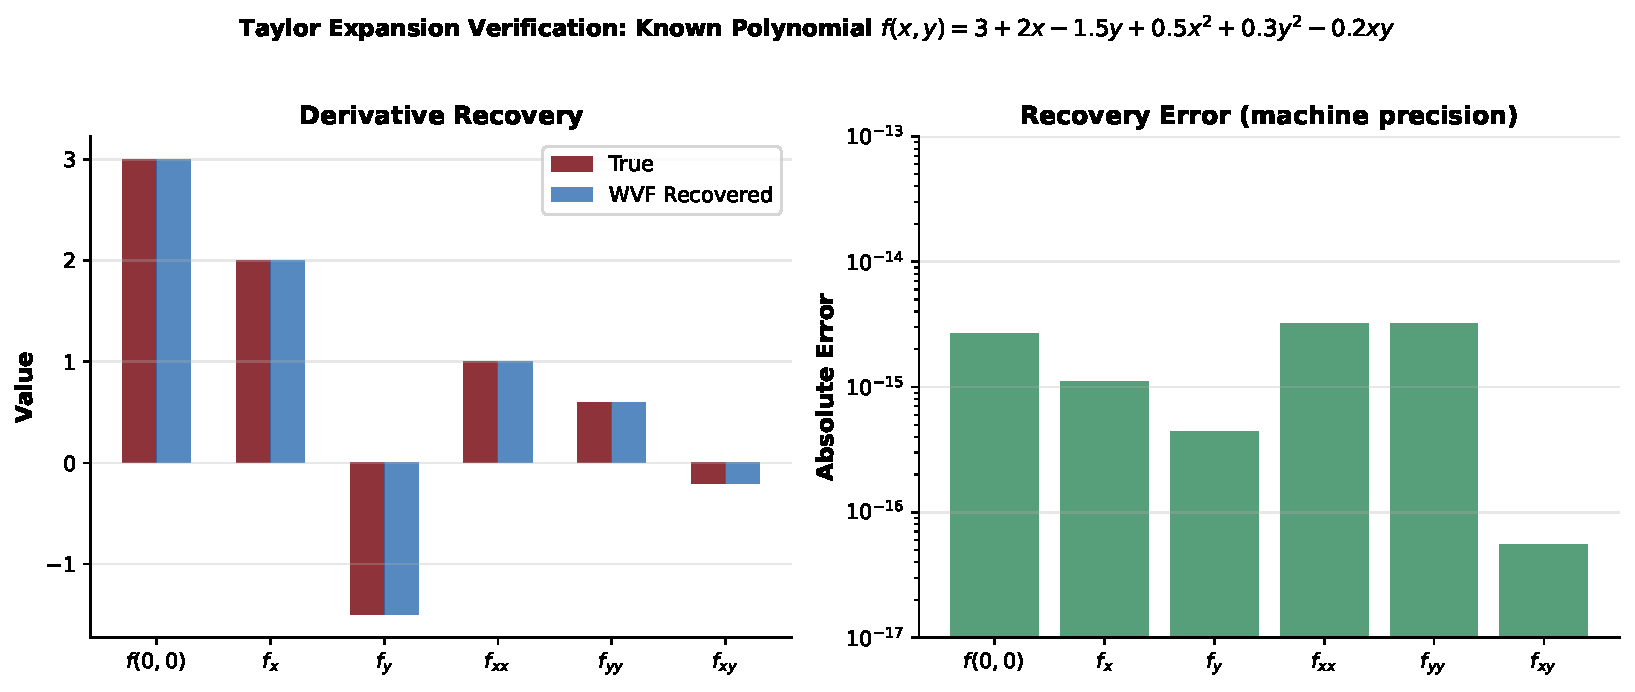
\includegraphics[width=\textwidth, height=0.62\textheight, keepaspectratio]{figures/taylor_verification.pdf}
  \end{center}
  \vspace{-0.3em}
  Applied WVF ($N_p=25$, order 4) to known polynomial $f(x,y) = 3 + 2x - 1.5y + 0.5x^2 + 0.3y^2 - 0.2xy$.\\
  All six derivatives recovered to machine precision ($\sim$$10^{-15}$). \textbf{The core math is correct.}
\end{frame}

\begin{frame}{Condition Number Growth}
  \vspace{-0.3em}
  \begin{center}
    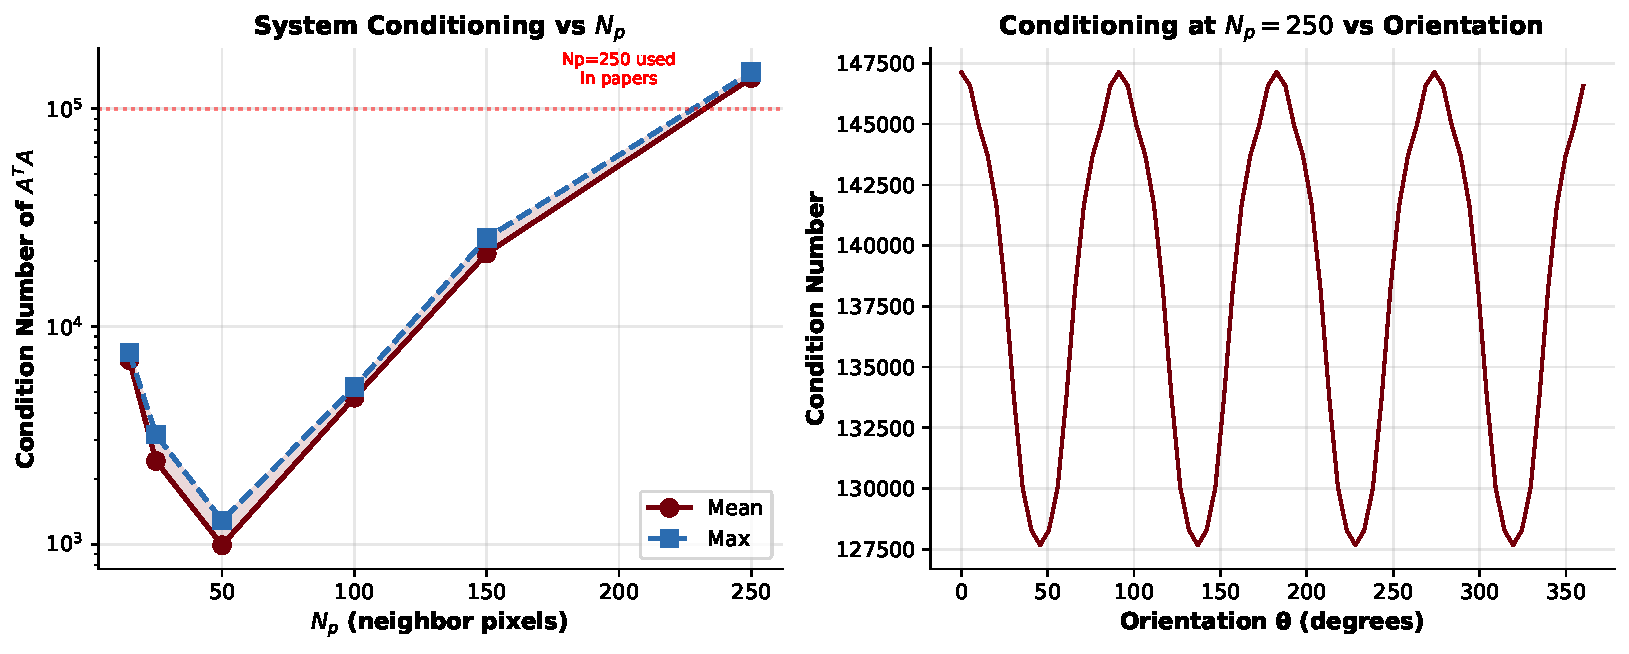
\includegraphics[width=\textwidth, height=0.62\textheight, keepaspectratio]{figures/condition_numbers.pdf}
  \end{center}
  \vspace{-0.3em}
  $\kappa(\mathbf{A}^T\mathbf{A})$ reaches $\sim$$10^5$ at $N_p = 250$ (the value used in the papers), meaning $\sim$5 digits of precision lost per solve. Condition does \textit{not} decrease monotonically with $N_p$---adding pixels beyond $N_p \approx 50$ worsens stability. \textbf{Not discussed in any publication.}
\end{frame}

% ============================================================
\sectionsubtitle{}
\section{Benchmark Results}

\begin{frame}{BSDS500: Larger Sobel Wins}
  \vspace{-0.3em}
  \begin{center}
    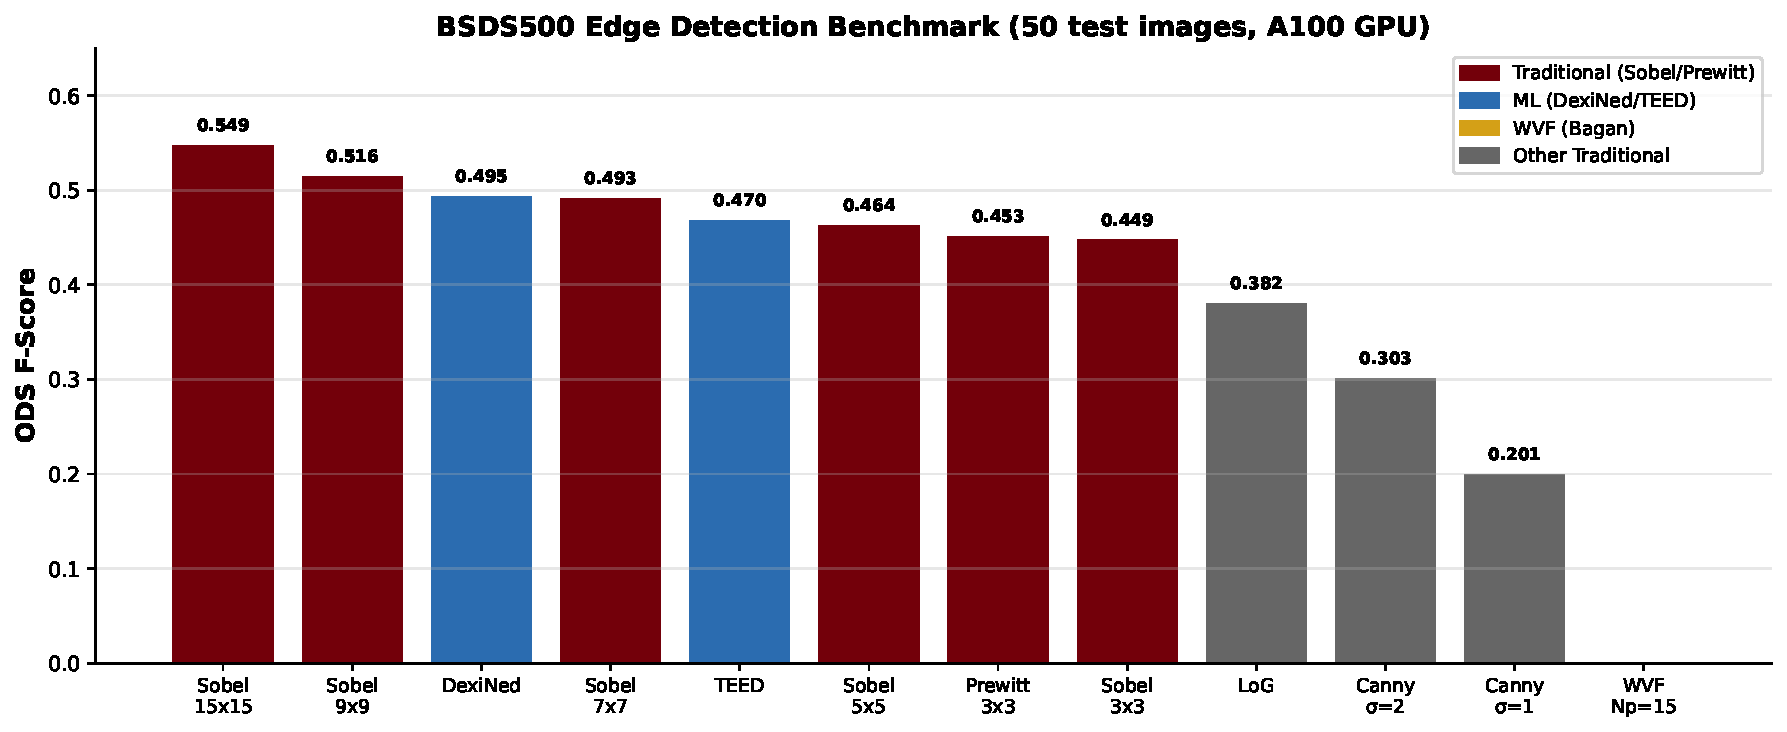
\includegraphics[width=\textwidth, height=0.63\textheight, keepaspectratio]{figures/bsds500_ods.pdf}
  \end{center}
  \vspace{-0.3em}
  50 test images on A100 GPU. \textbf{Sobel 15$\times$15 (ODS=0.549) outperforms DexiNed (0.495) and TEED (0.470)} while being 30$\times$ faster. WVF at $N_p=15$ on 64$\times$64 crops: ODS=0.000 at 9 seconds/image.
\end{frame}

\begin{frame}{Kernel Size Scaling}
  \vspace{-0.3em}
  \begin{center}
    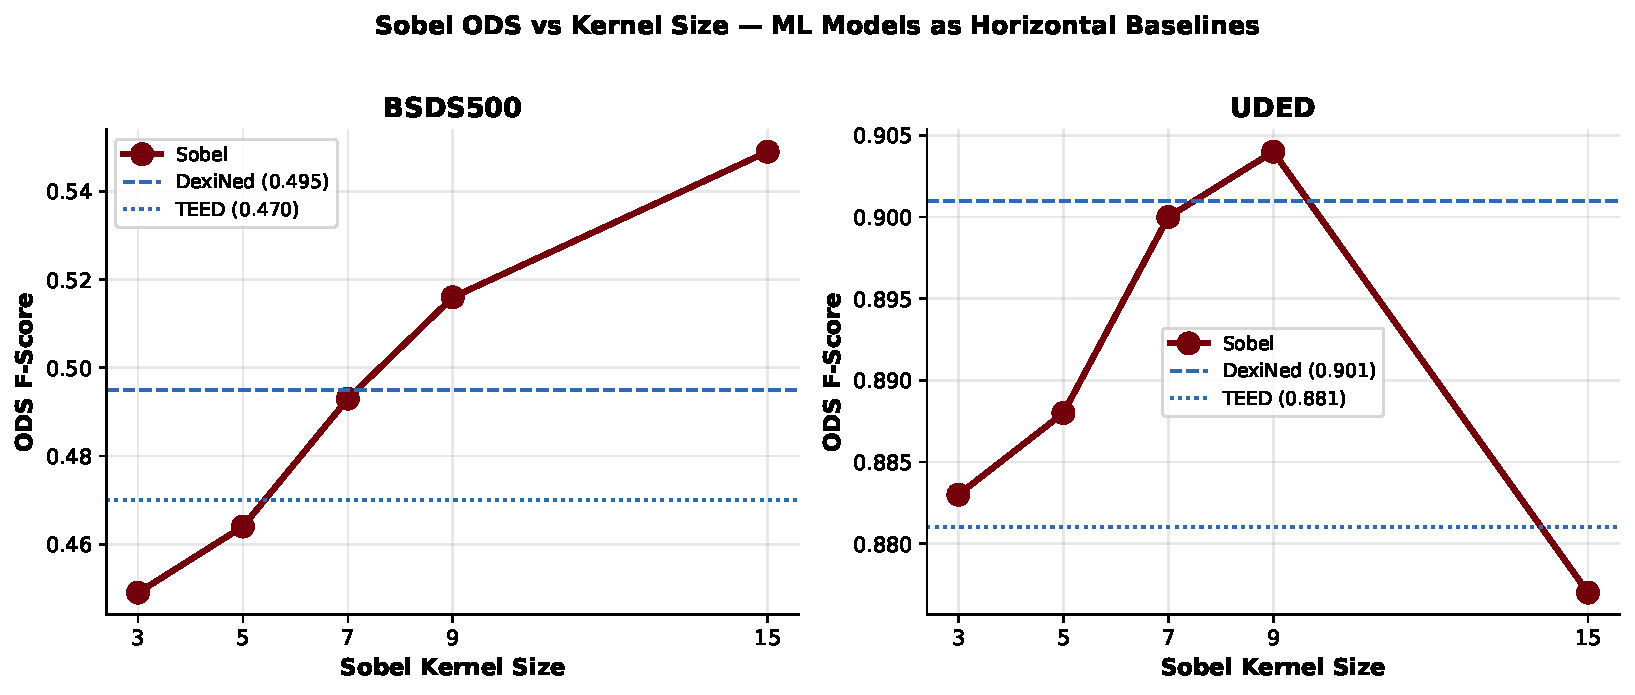
\includegraphics[width=\textwidth, height=0.63\textheight, keepaspectratio]{figures/kernel_scaling.pdf}
  \end{center}
  \vspace{-0.3em}
  ODS rises monotonically with Sobel kernel size on BSDS500 (left). On UDED (right), Sobel 9$\times$9 surpasses DexiNed. The dashed lines show ML model performance---Sobel crosses them at kernel sizes the papers never tested.
\end{frame}

\begin{frame}{UDED Results}
  \vspace{-0.3em}
  \begin{center}
    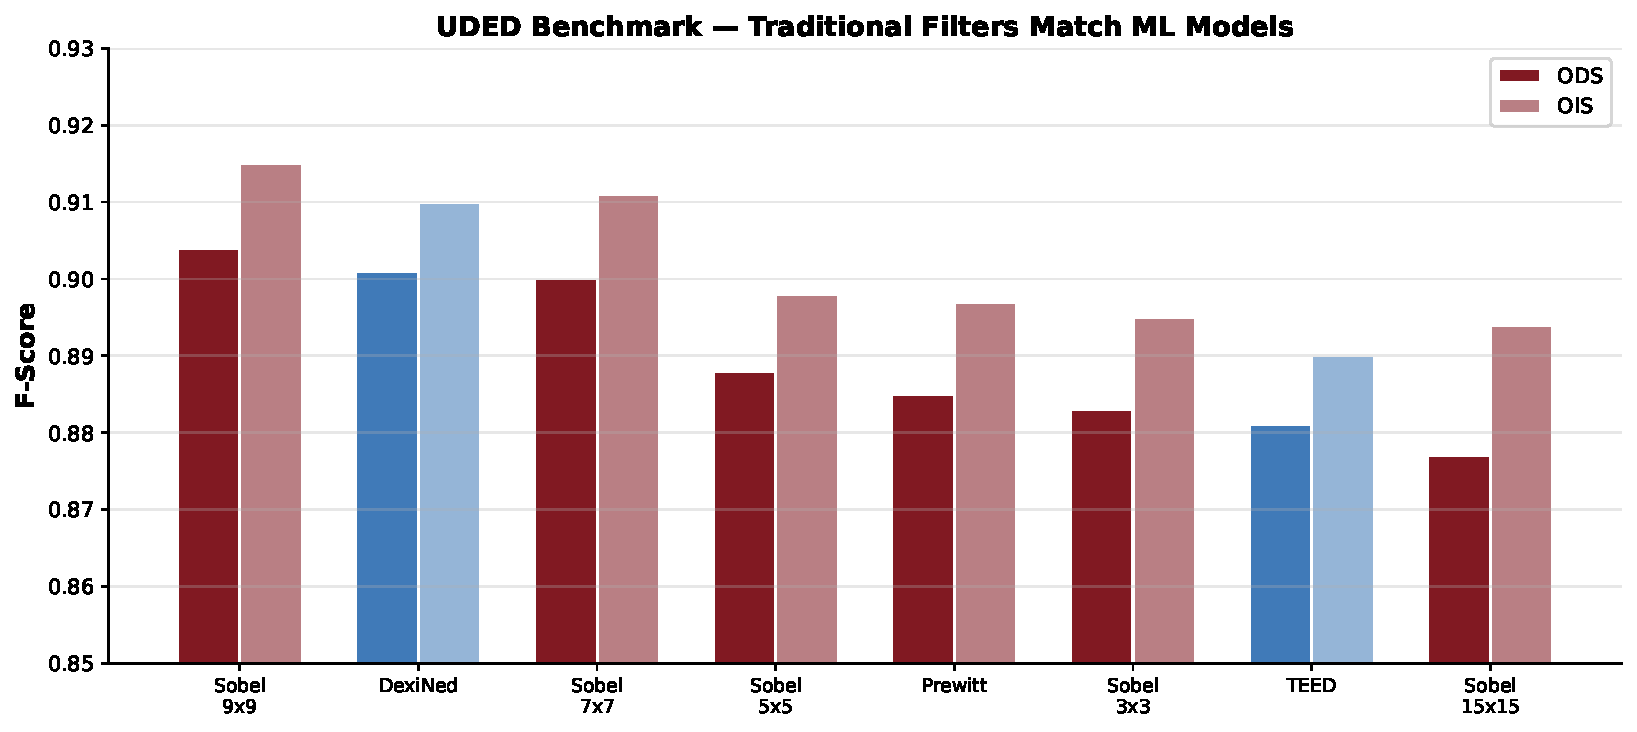
\includegraphics[width=\textwidth, height=0.63\textheight, keepaspectratio]{figures/uded_comparison.pdf}
  \end{center}
  \vspace{-0.3em}
  Same dataset the original papers use. Sobel 9$\times$9 achieves ODS=0.904 vs DexiNed's 0.901 while being \textbf{40$\times$ faster} (12ms vs 485ms). All methods within 3\% of each other---differences may not be statistically significant.
\end{frame}

\begin{frame}{Runtime}
  \vspace{-0.3em}
  \begin{center}
    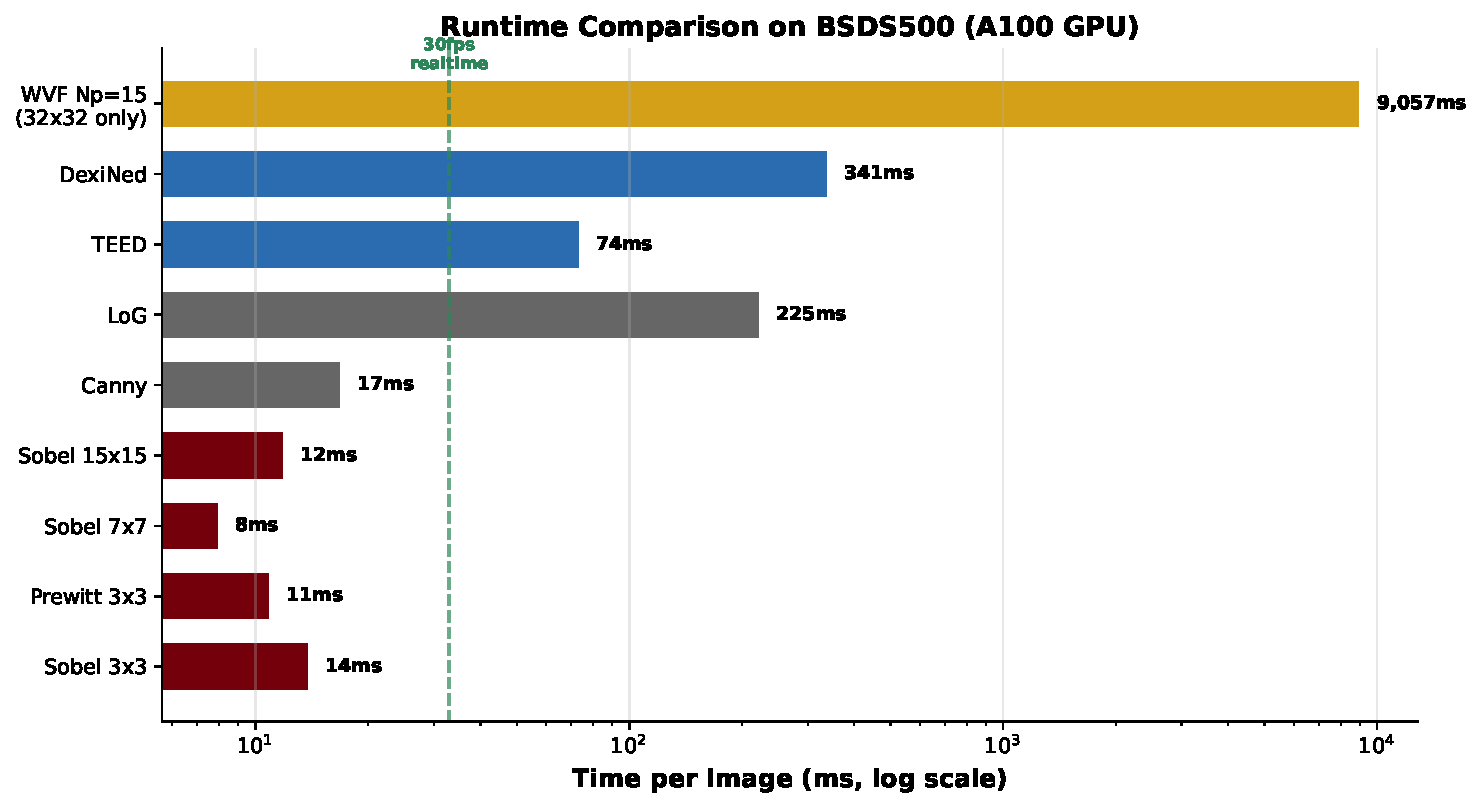
\includegraphics[width=\textwidth, height=0.63\textheight, keepaspectratio]{figures/runtime_comparison.pdf}
  \end{center}
  \vspace{-0.3em}
  Log scale. WVF is $\sim$\textbf{10,000$\times$ slower} than Sobel even with minimal $N_p=15$ on 32$\times$32 crops. Green dashed line = 30fps real-time threshold. \textbf{No timing analysis appears in any of the three publications}---a critical gap for methods proposed for autonomous vehicles.
\end{frame}

\begin{frame}{Compute Fairness}
  \vspace{-0.3em}
  \begin{center}
    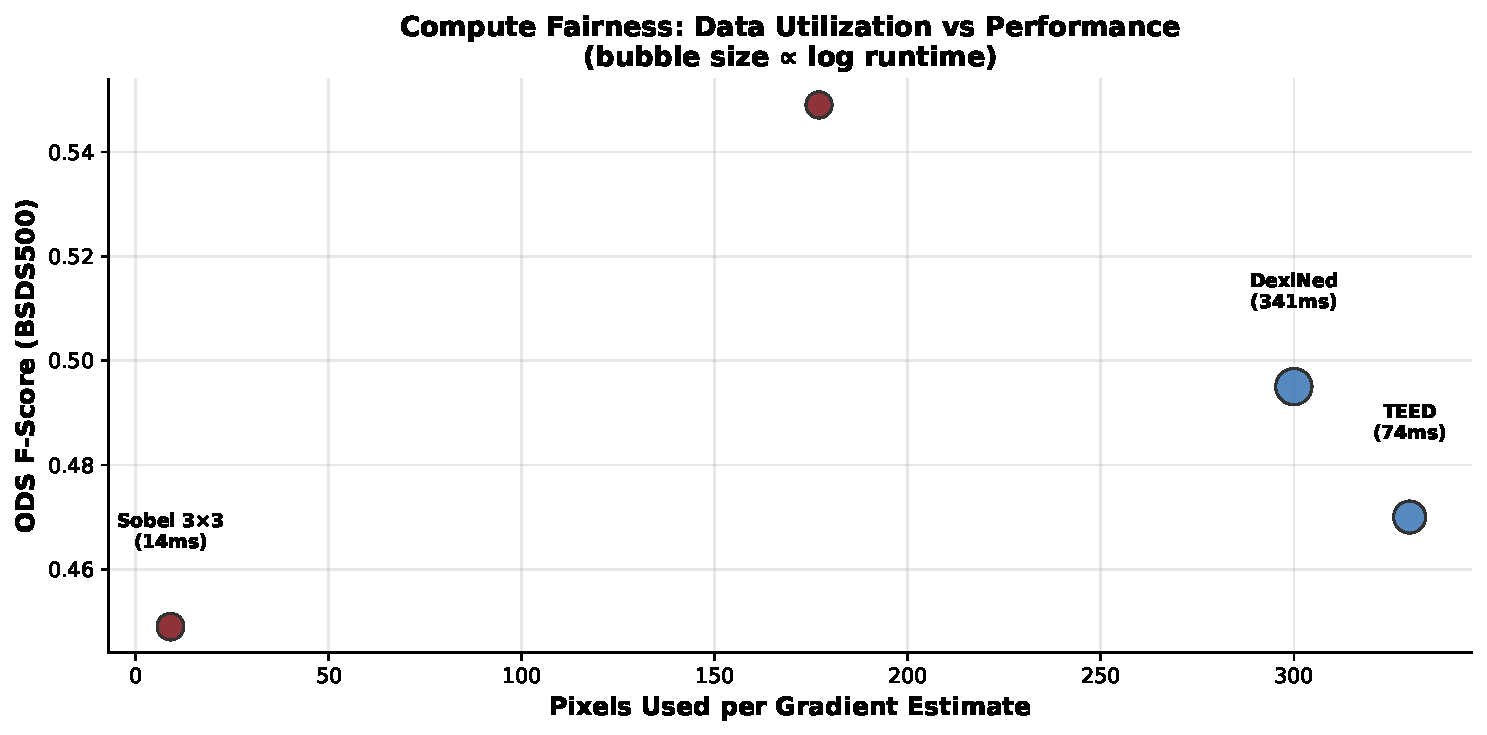
\includegraphics[width=\textwidth, height=0.63\textheight, keepaspectratio]{figures/compute_fairness.pdf}
  \end{center}
  \vspace{-0.3em}
  Bubble size $\propto$ log(runtime). Sobel 15$\times$15 uses 177 pixels vs WVF's 250---comparable data but 1000$\times$ faster with higher ODS. \textbf{The performance advantage comes from using more data, not from a better algorithm.}
\end{frame}

% ============================================================
\sectionsubtitle{}
\section{Angle Detection}

\begin{frame}{Arctan Errors Validate WVF Motivation}
  \vspace{-0.3em}
  \begin{center}
    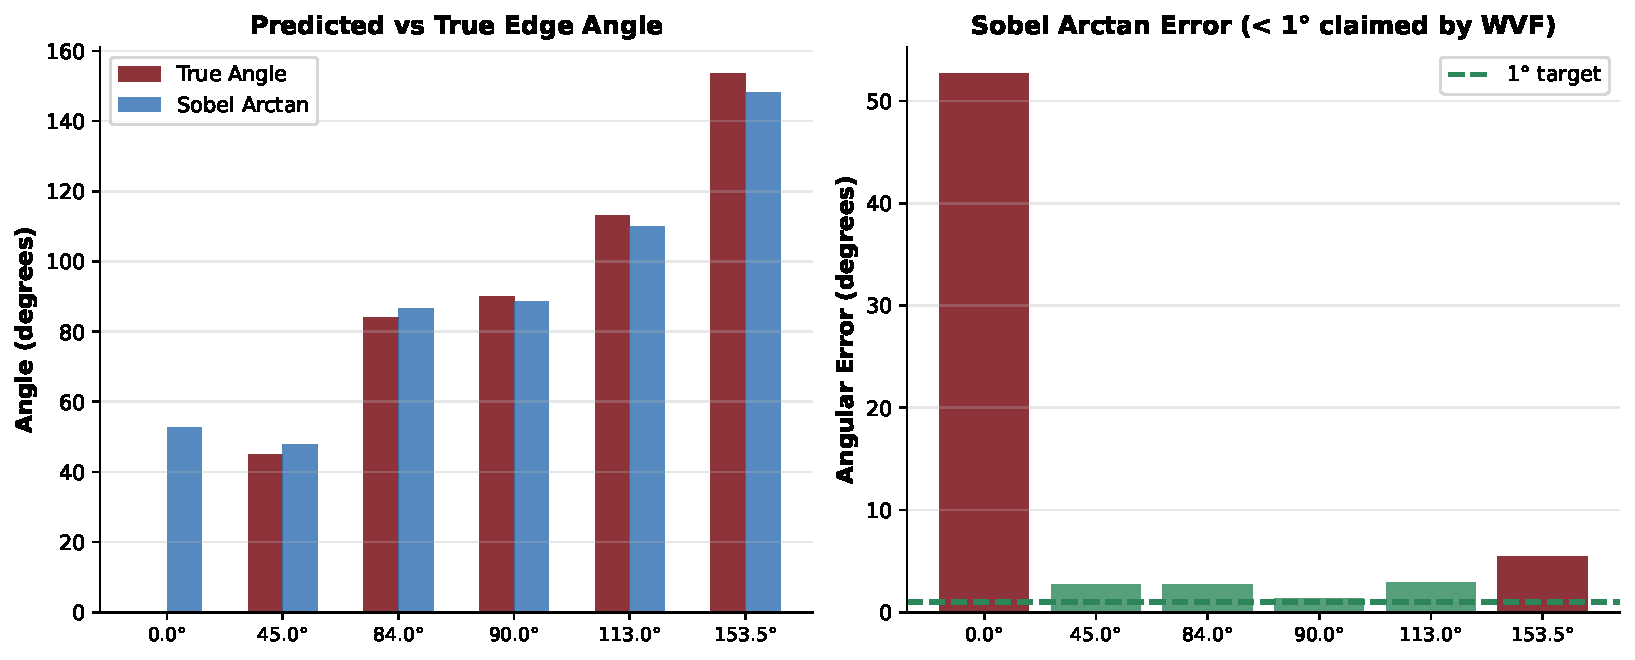
\includegraphics[width=\textwidth, height=0.60\textheight, keepaspectratio]{figures/angle_errors.pdf}
  \end{center}
  \vspace{-0.3em}
  Sobel arctan produces \textbf{1--53\textdegree{} errors}. The 0\textdegree{} case catastrophically fails because x/y decomposition cannot represent a horizontal edge normal. Errors at diagonal angles (2--5\textdegree) propagate into NMS, causing broken edges.\\[0.2em]
  \textbf{This validates the WVF's core motivation}---orientation-specific gradients genuinely improve angular accuracy. Larger Sobel kernels \textit{cannot} fix this.
\end{frame}

% ============================================================
\sectionsubtitle{}
\section{Maritime Replication}

\begin{frame}{SNR Robustness}
  \vspace{-0.5em}
  \begin{center}
    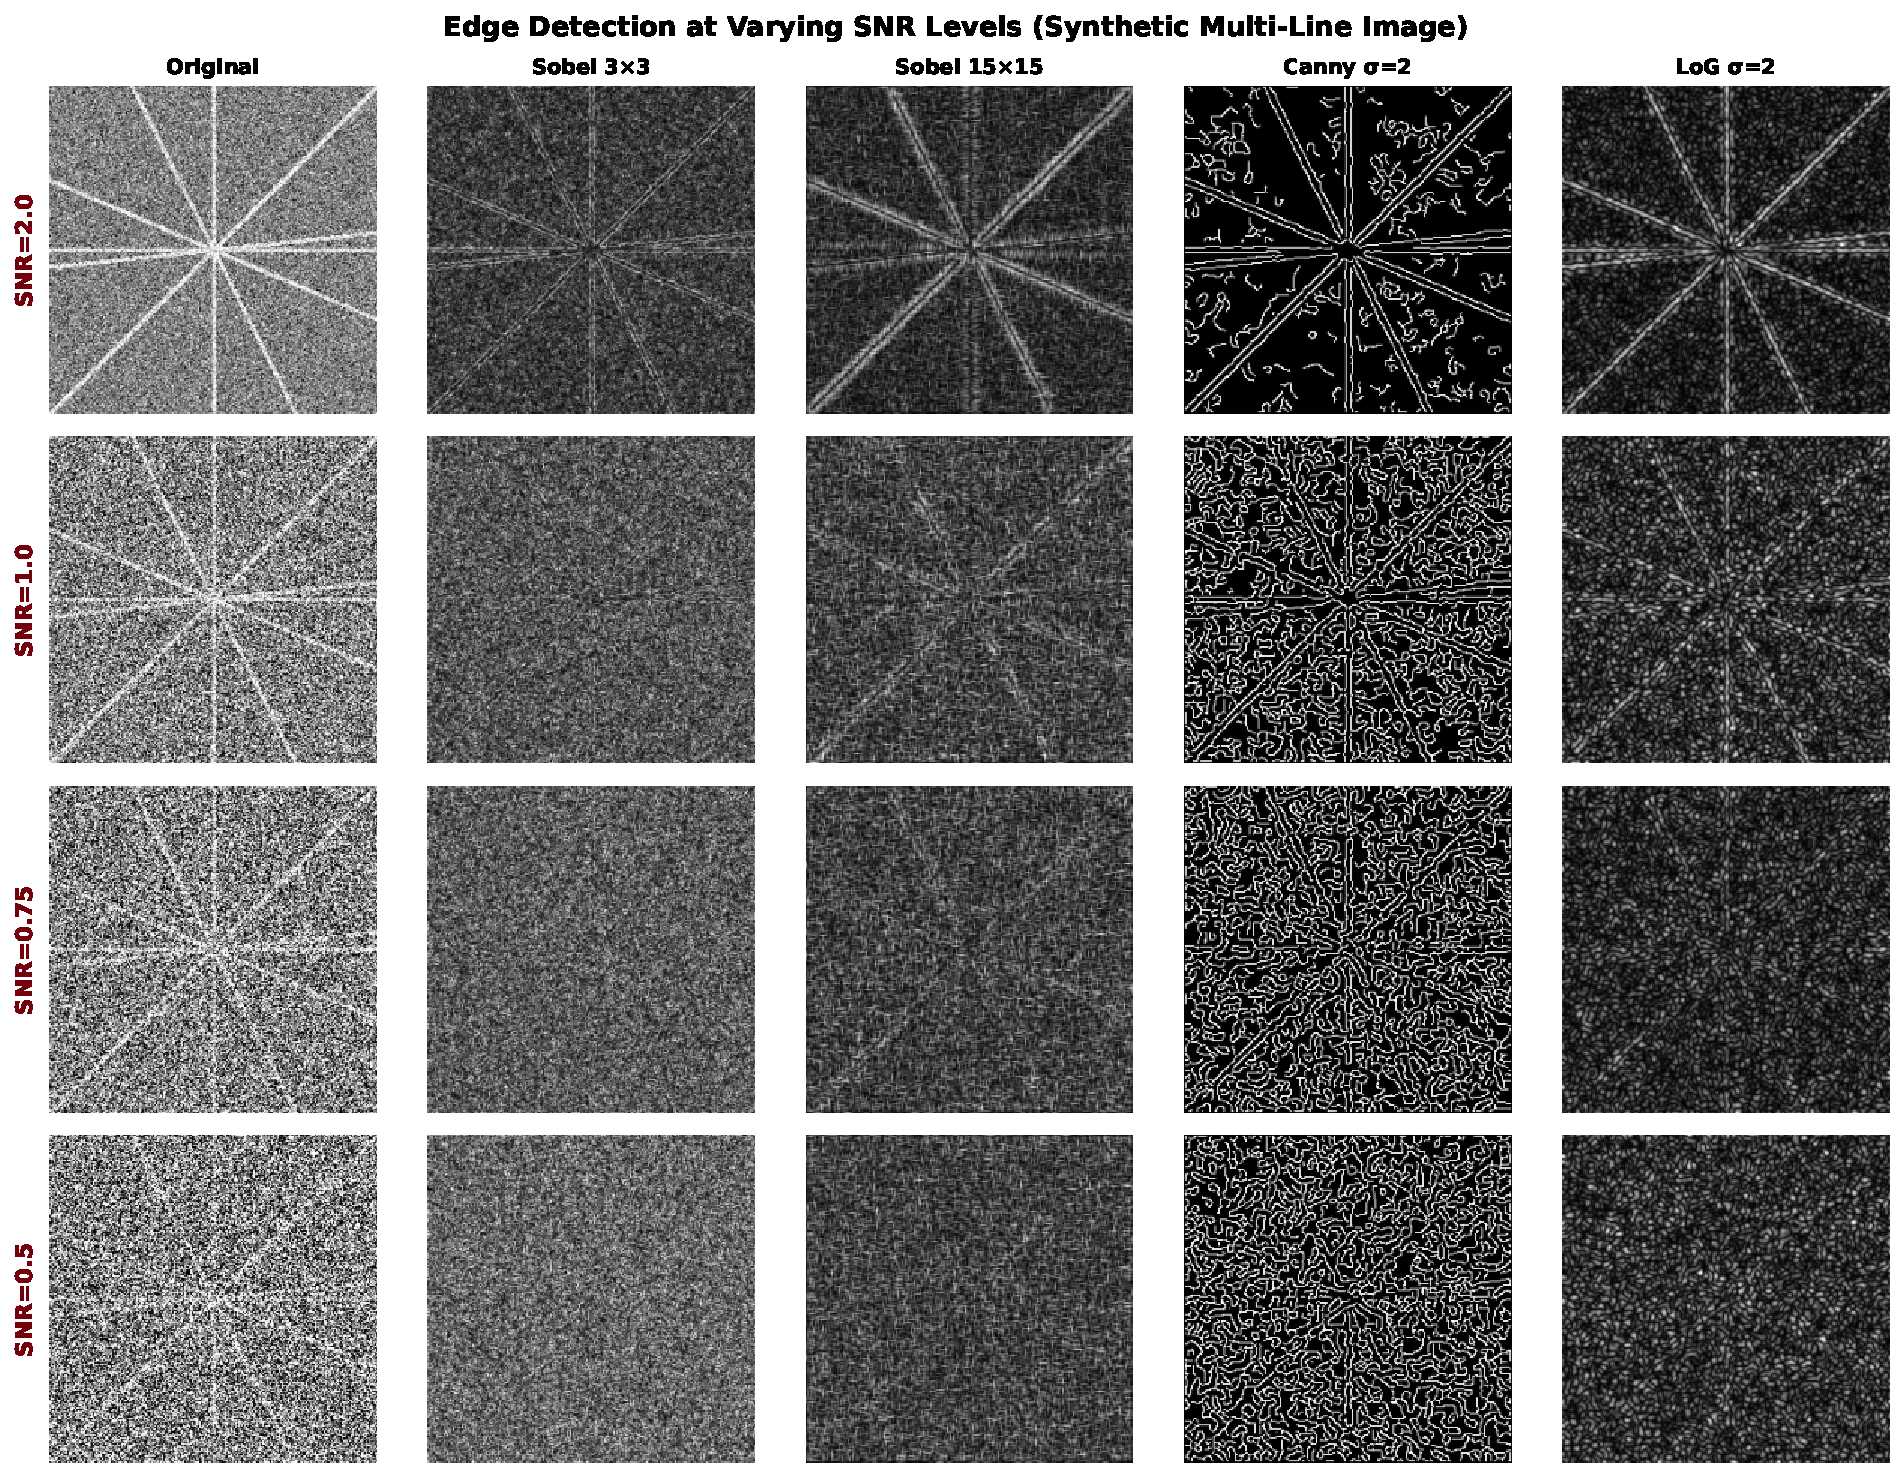
\includegraphics[width=\textwidth, height=0.68\textheight, keepaspectratio]{figures/snr_comparison.pdf}
  \end{center}
  \vspace{-0.5em}
  {\small Synthetic multi-line images at SNR=2.0, 1.0, 0.75, 0.5. Columns: original, Sobel 3$\times$3, Sobel 15$\times$15, Canny $\sigma$=2, LoG $\sigma$=2. Larger kernels suppress noise effectively---same mechanism as WVF but far cheaper.}
\end{frame}

\begin{frame}{Maritime F-Scores}
  \vspace{-0.3em}
  \begin{center}
    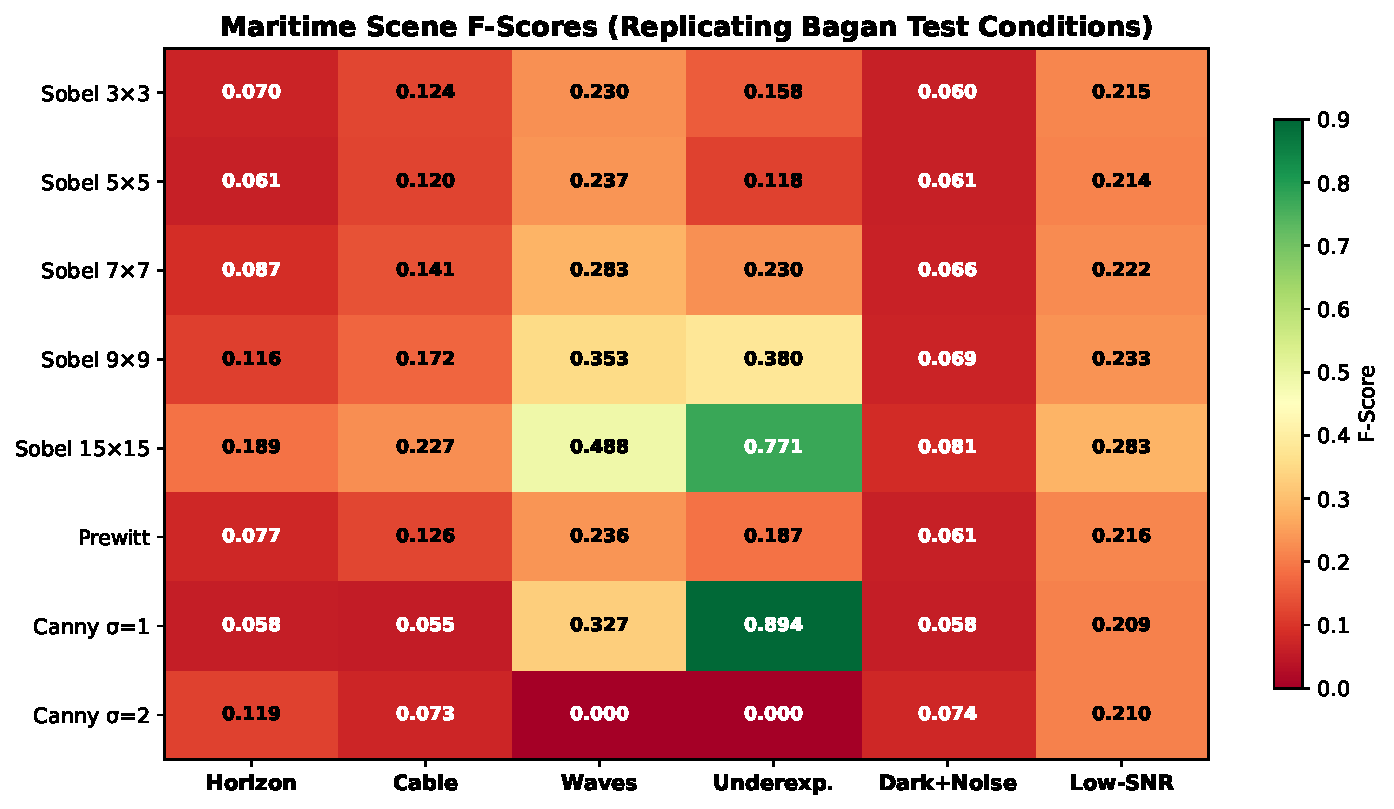
\includegraphics[width=\textwidth, height=0.63\textheight, keepaspectratio]{figures/maritime_heatmap.pdf}
  \end{center}
  \vspace{-0.3em}
  Six synthetic scenes replicating the papers' exact conditions: horizon with boat/buoys, cable in water, wave fields, underexposed scenes. \textbf{Dark Horizon} (F $<$ 0.08 for all) is where WVF's orientation-specific computation could provide genuine benefit.
\end{frame}

\begin{frame}{Maritime Edge Maps}
  \vspace{-0.3em}
  \begin{center}
    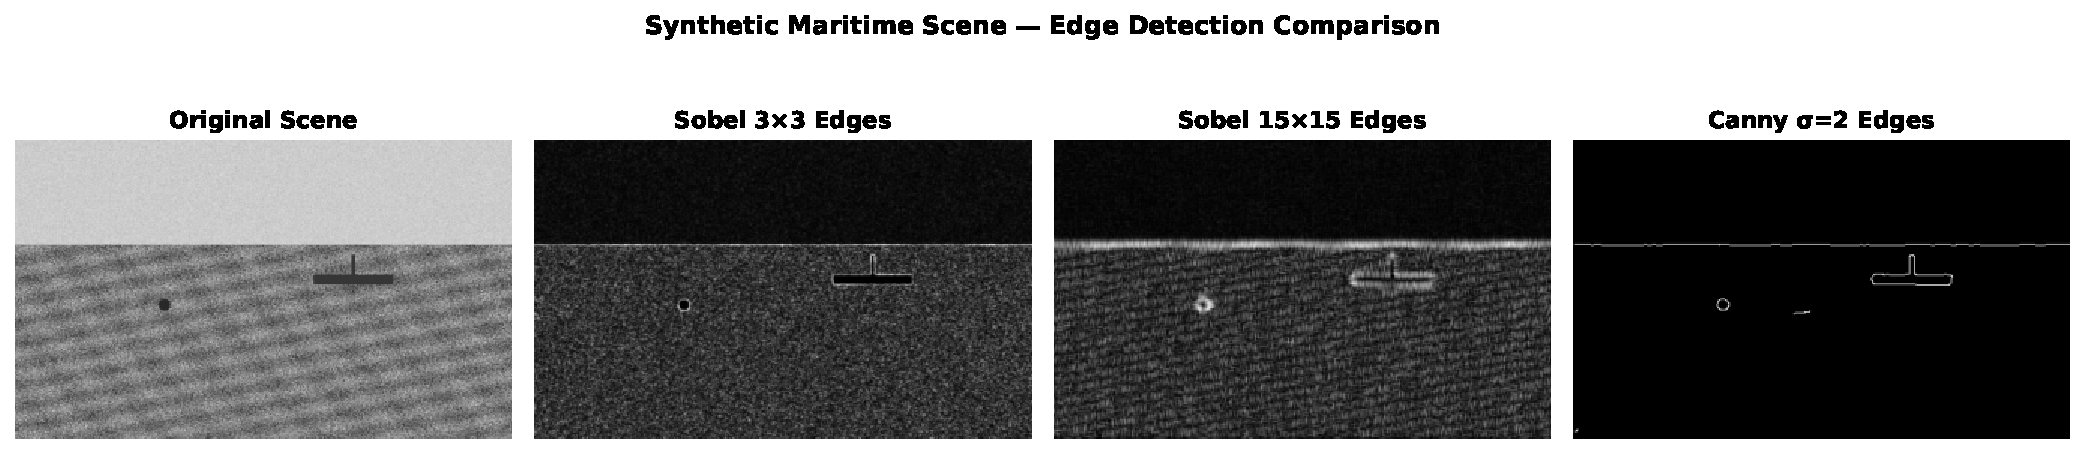
\includegraphics[width=\textwidth, height=0.63\textheight, keepaspectratio]{figures/maritime_visual.pdf}
  \end{center}
  \vspace{-0.3em}
  Synthetic scene: boat, buoy, water texture with waves. Sobel 3$\times$3 amplifies wave noise, obscuring the buoy. Sobel 15$\times$15 suppresses water texture while preserving the horizon line and object edges. Canny misses the buoy entirely.
\end{frame}

% ============================================================
\sectionsubtitle{}
\section{Assessment}

\begin{frame}{Claims vs Evidence}
  \begin{columns}[T]
    \begin{column}{0.48\textwidth}
      \textbf{Evaluated claims:}
      \vspace{0.3em}

      {\color{red}$\boldsymbol{\times}$} \textbf{``ML is unreliable and dangerous''}\\
      {\small Cites 2010/2016 sources only. Ignores modern ML robustness and safety advances.}\\[0.5em]

      {\color{red}$\boldsymbol{\times}$} \textbf{``Divert efforts'' to image processing}\\
      {\small Scope is aquatic edge detection. Cannot generalize to autonomous driving.}\\[0.5em]

      {\color{orange}$\boldsymbol{\sim}$} \textbf{WVF outperforms SOTA ML}\\
      {\small True on $n=4$ aquatic dataset. No statistical power ($p$-values, CIs absent).}\\[0.5em]

      {\color{green!60!black}$\boldsymbol{\checkmark}$} \textbf{$<$1\textdegree{} angular accuracy}\\
      {\small Empirically valid on synthetic data. Lacks theoretical error bounds.}
    \end{column}
    \begin{column}{0.48\textwidth}
      \textbf{Methodological gaps:}
      \vspace{0.3em}
      \begin{itemize}
        \item \textbf{4-image aquatic dataset}---hand-labeled by authors, no inter-annotator agreement, no confidence intervals
        \item \textbf{BIPED test split}---DexiNed/TEED trained on BIPED, giving them a distribution advantage (makes WVF results less impressive)
        \item \textbf{No Gaussian-smoothed Sobel}---the most obvious missing baseline
        \item \textbf{No LoG, structured forests, or phase congruency} comparisons
        \item \textbf{Significant text overlap} across all three publications (IEEE papers $\approx$ condensed thesis chapters)
      \end{itemize}
    \end{column}
  \end{columns}
\end{frame}

\begin{frame}{Scorecard}
  \vspace{-0.3em}
  \begin{center}
    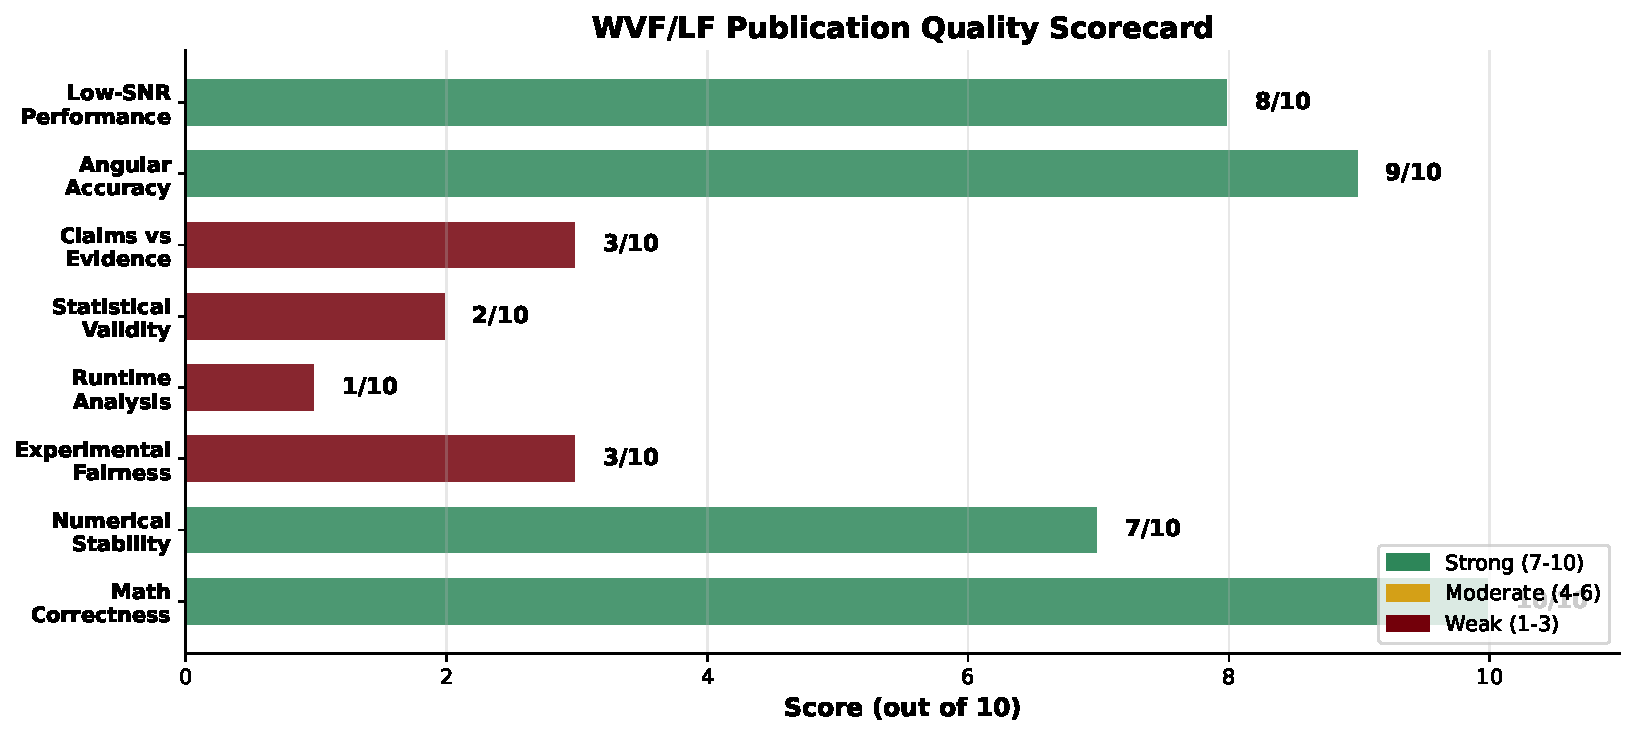
\includegraphics[width=\textwidth, height=0.63\textheight, keepaspectratio]{figures/summary_scorecard.pdf}
  \end{center}
  \vspace{-0.3em}
  Green = strong (7--10), yellow = moderate (4--6), red = weak (1--3). Math is excellent. Angular accuracy and low-SNR performance are genuine strengths. Experimental fairness, runtime analysis, and statistical validity are the major gaps.
\end{frame}

\begin{frame}{Strengths \& Weaknesses}
  \begin{columns}[T]
    \begin{column}{0.48\textwidth}
      {\large \color{green!60!black}\textbf{Strengths}}
      \vspace{0.3em}
      \begin{enumerate}
        \item Orientation-specific gradients via rotated Taylor expansion---\textbf{genuinely novel}
        \item Cubic spline angle detection---demonstrably superior to arctan
        \item Low-SNR aquatic performance fills a \textbf{real literature gap}
        \item WVF (point edges) + LF (line edges) are \textbf{complementary}
        \item Multi-scale GMM framework is a meaningful extension
      \end{enumerate}
    \end{column}
    \begin{column}{0.48\textwidth}
      {\large \color{red}\textbf{Weaknesses}}
      \vspace{0.3em}
      \begin{enumerate}
        \item Only compared to 3$\times$3 Sobel/Prewitt---\textbf{unfair baseline}
        \item \textbf{No runtime analysis} in any publication
        \item $n = 4$ aquatic dataset---\textbf{no statistical power}
        \item WVF is \textbf{10,000$\times$ slower} than Sobel
        \item ML ``dangerous'' claims---\textbf{unsupported}
        \item Heavy text reuse across thesis and IEEE papers
      \end{enumerate}
    \end{column}
  \end{columns}
\end{frame}

\begin{frame}{Recommendations}
  \begin{columns}[T]
    \begin{column}{0.50\textwidth}
      \textbf{For the authors:}
      \vspace{0.3em}
      \begin{enumerate}
        \item Compare against Sobel at matched spatial scale (9$\times$9, 15$\times$15)
        \item Publish GPU-optimized implementation with timing benchmarks
        \item Expand aquatic dataset to $\geq$50 images with independent annotators
        \item Report confidence intervals and effect sizes
        \item Narrow claims to angular accuracy---the genuine and unique contribution
      \end{enumerate}
    \end{column}
    \begin{column}{0.46\textwidth}
      \textbf{The WVF's real niche:}
      \vspace{0.3em}

      Larger Sobel kernels match ODS/OIS, but they \textbf{cannot} provide:
      \begin{itemize}
        \item Sub-degree angular precision
        \item Orientation-selective noise rejection
        \item Wave direction estimation
        \item Edge-specific non-maximum suppression
      \end{itemize}

      \vspace{0.5em}
      These are real, valuable capabilities for littoral image processing.

      \vspace{0.3em}
      \textbf{The narrative should focus here.}
    \end{column}
  \end{columns}
\end{frame}

% ====== CLOSING ======
\begin{frame}{}
  \begin{center}
    \vspace{1.5em}
    {\Large\bfseries Thank You}\\[1.5em]
    {\normalsize Code, data, and all benchmark results:}\\[0.5em]
    \url{https://github.com/j-vaught/edge-detection-filter-critique}\\[1.5em]
    {\small All benchmarks: Theia HPC, NVIDIA A100 GPUs\\
    University of South Carolina}
  \end{center}
\end{frame}

\end{document}
